% F5 — P6 daily train/evaluate cadence as a simple UTC timeline.
% Standalone TikZ; caption lives in the chapter. Times from the deployment
% inventory (Table 4.1): forecast 06:00, reconcile 18:00, drift 19:00 (all daily).
\documentclass[tikz,border=8pt]{standalone}
\usetikzlibrary{arrows.meta}

\begin{document}
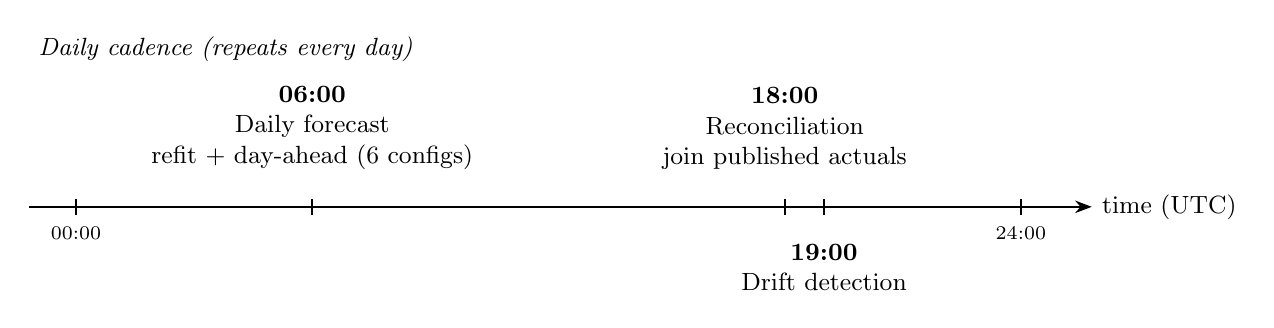
\begin{tikzpicture}[
  >={Stealth[length=6pt]},
  ev/.style={align=center, font=\small},
]
% axis
\draw[->, thick] (-0.6,0) -- (12.9,0) node[right, font=\small]{time (UTC)};
\foreach \x in {0,3,9,9.5,12}{ \draw[thick] (\x,0.1) -- (\x,-0.1); }
\node[font=\scriptsize, below=1pt] at (0,-0.1)  {00:00};
\node[font=\scriptsize, below=1pt] at (12,-0.1) {24:00};

% events
\node[ev, anchor=south] at (3,0.35)
   {\textbf{06:00} \\ Daily forecast \\ refit + day-ahead (6 configs)};
\node[ev, anchor=south] at (9,0.35)
   {\textbf{18:00} \\ Reconciliation \\ join published actuals};
\node[ev, anchor=north] at (9.5,-0.35)
   {\textbf{19:00} \\ Drift detection};

\node[font=\small\itshape, anchor=west] at (-0.6,2.0) {Daily cadence (repeats every day)};
\end{tikzpicture}
\end{document}
